\section{AE21B107}

\subsection*{\centering{Stefan-Boltzmann law}}

This law was formulated by Austrian physicist Josef Stefan in 1879 as a result of experimental studies. The same law, in 1884, was derived by Austrian physicist Ludwig Boltzmann from thermodynamic considerations.

Stefan-Boltzmann law states that the total radiant heat energy emitted per unit time from a surface is proportional to the fourth power of its temperature (in Kelvins i.e. Absolute temperature).

The emissivity of blackbody, a theoretical body considered to absorb all radiations incident on it, is 1 and that for ordinary body is between 0 and 1.

\begin{equation}
    \text{E} = {\sigma}{eT^4} 
\end{equation}

where $\sigma$ is known as Stefan-Boltzmann constant.

\begin{equation*}
      {\sigma} = 5.67 \times 10^{-8}
\end{equation*}

Other forms of this equation can be represented as,

\begin{equation}
    \frac{dq}{dt} = {\sigma}{eT^4}
\end{equation}

\begin{equation}
    \frac{dQ}{dt} = {\sigma}{eAT^4}
\end{equation}

The symbols used are as follows,

\begin{table}[h]
    \centering
    \begin{tabular}{|c|l|}
    \hline
    E & Radiant heat energy emitted per unit area per second \\
    q & Radiant heat energy per unit area \\
    Q & Radiant heat energy\\
    A & Area of the radiant surface\\
    T & Absolute Temperature of the body\\
    e & Emissivity of the body\\
    $\sigma$ & Stefan-Boltzmann constant \\
    \hline
    \end{tabular}
    \caption{Symbols used in above representations of Stefan-Boltzmann law}
\end{table}

The following plots show the variation of E vs T for a given body with e = 1 in Graph 1 and variation of E vs T for various values of e in graph 2.

\includegraphics[scale=0.6]{jan-may-2022-latex/AE21B107/EvsT.png}
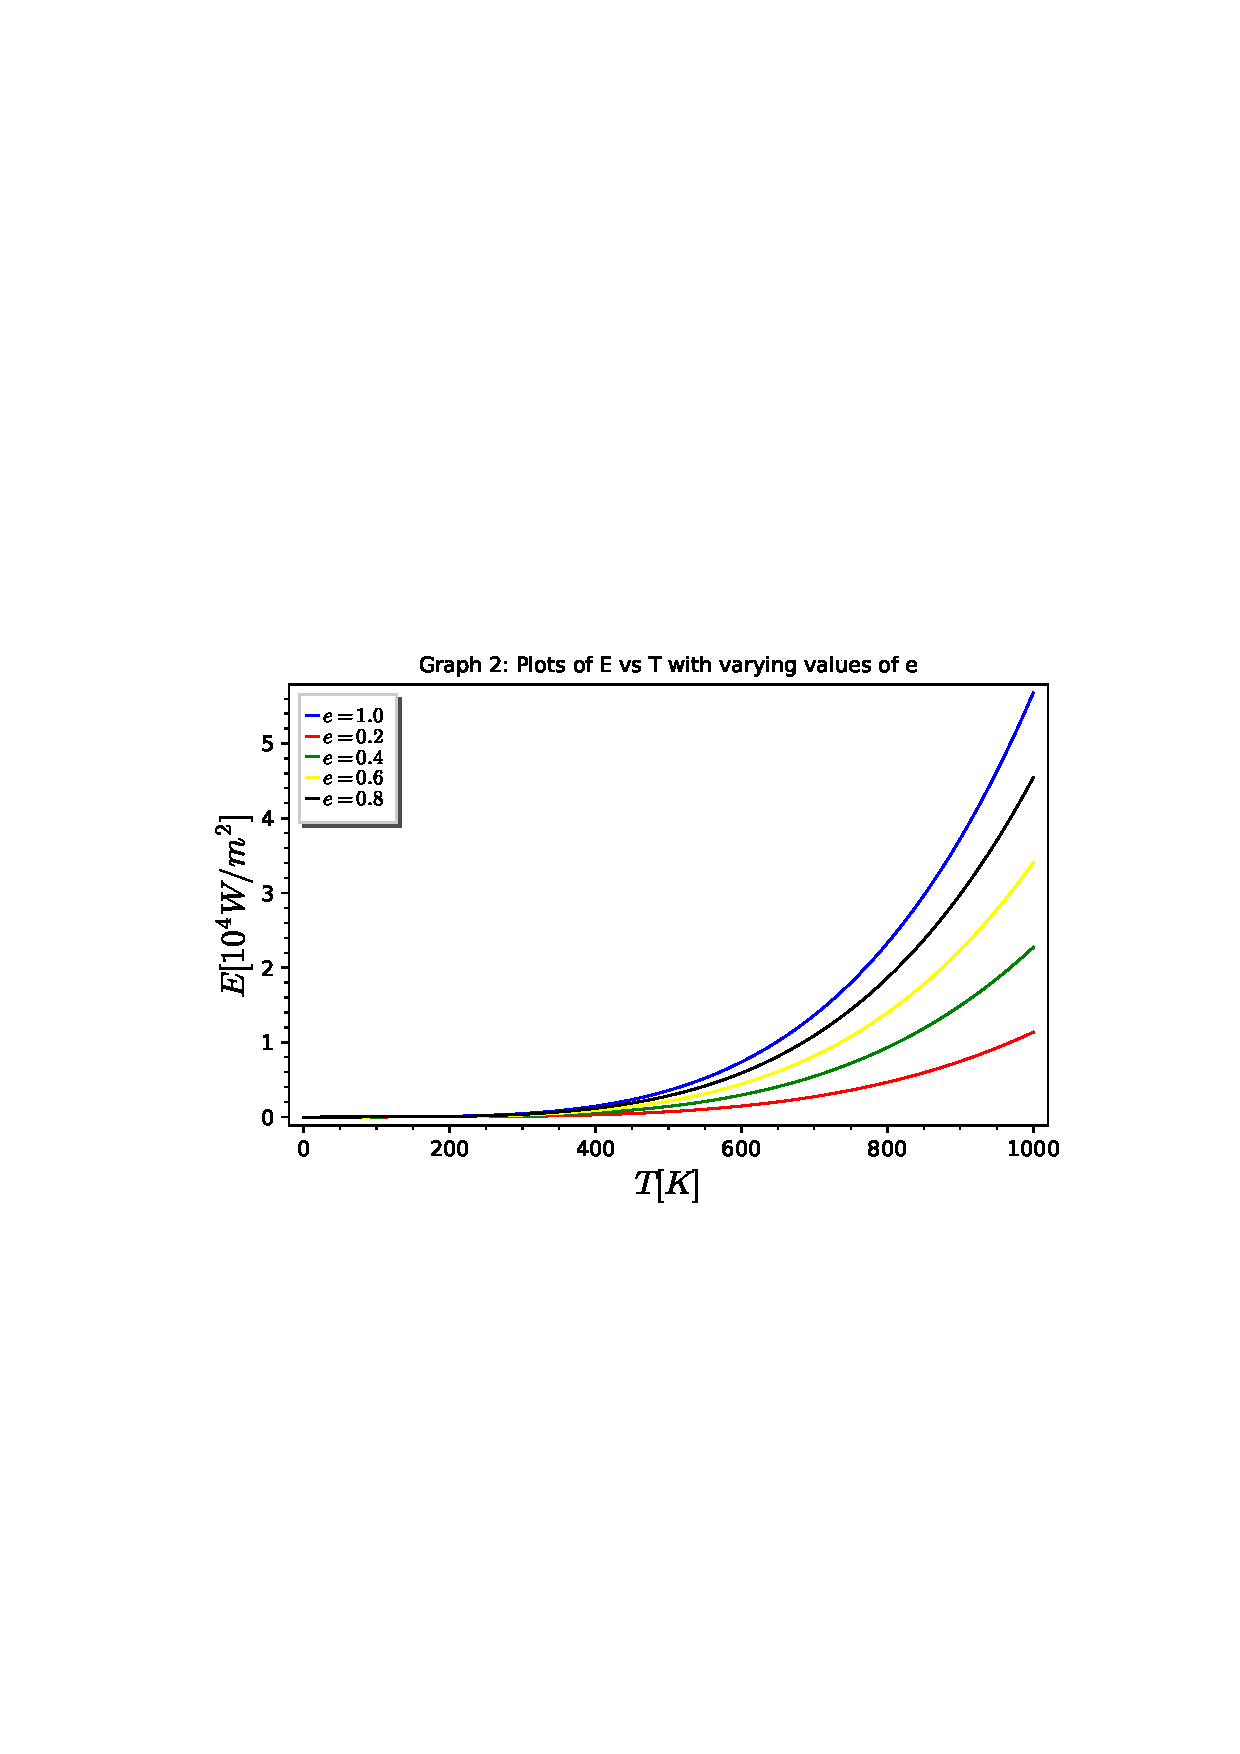
\includegraphics[scale=0.6]{jan-may-2022-latex/AE21B107/variable_e.png}
